\section{Open vs Closed loop identification}
In this experiment we had the necessity to choose whether to consider back-emf in the identification process or to completely ignore it. \\
As a matter of fact, ignoring it would mean to neglect a feedback component. But how much can it affect identification of other parameters?
\\ \\
Consider for example the following 2-nd order system, such as the system considered in the experiment:
$$G(s) = \frac{1}{Ms^2+cs+k}$$
\\ \\
First consider a feedback loop with a constant gain $\rho$ on the feedback. Thus the closed loop transfer function is:
$$T(s) = \frac{G(s)}{1+\rho G(s)} = \frac{1}{Ms^2+cs+(k+\rho )}$$
The effect of $\rho$ is to change the length of the poles, i.e. their absolute value, since for polynomial with real coefficients the zero-degree coefficient is the product of all roots. \\
Just compare with $s^2+2\xi \omega_0 s+ \omega_0^2$, it's easy to see that $\omega_0^2 = \frac{k+\rho}{M}$.
\\\ \\
In our case  back-emf acts on the velocity of the cart, so if we have a feedback loop on the position, on the feedback we have  $\gamma s$, and the  closed loop transfer function is:
$$T(s) = \frac{1}{Ms^2+cs+k+\gamma s}$$
So what is the effect of $\gamma s$?
Again, if we compare with $s^2+2\xi \omega_0 s+ \omega_0^2$ we have:
$$c+\gamma = 2\xi \omega_0$$
Where $\xi$ has a strict relationship with the angle formed between the real negative axis and a pole,  $\theta$ :
$$\theta = \arctan \Big(\frac{\sqrt{1-\xi^2}}{\xi} \Big)$$
So the effect of $\gamma s$ is to rotate the poles, but to which extent is this effect negligible? \\ \\
From data we are mainly dealing with values of $\xi \in (0, 0.5)$, so we can approximate the value of $\theta$:
$$\theta \approx \arctan \Big(\frac{1-\frac{\xi^2}{2}}{\xi} \Big) = \arctan \Big(\frac{1}{\xi}-\frac{\xi}{2} \Big) \approx \arctan \Big (\frac{1}{\xi} \Big)$$
\begin{figure}
\centering
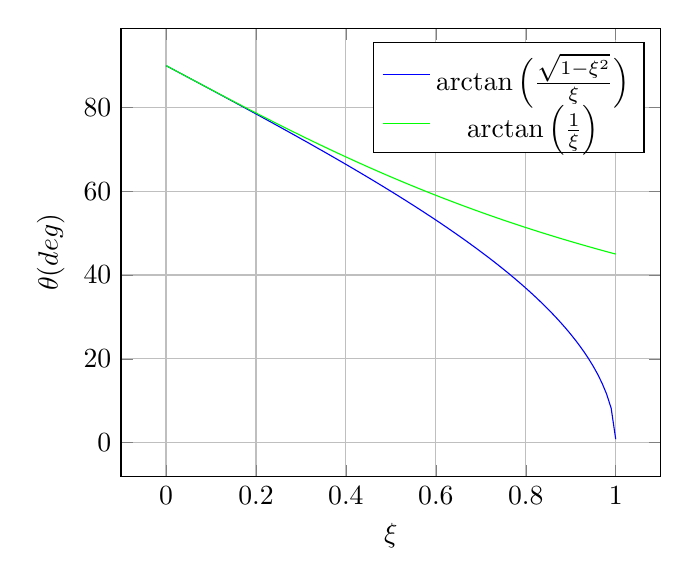
\begin{tikzpicture}
\begin{axis}[domain=0:1, samples=100,grid=major,
    restrict y to domain=0:90,xlabel=$\xi$,ylabel=$\theta (deg)$, legend pos=north east]
\addplot [color=blue] {atan( sqrt(1-x^2)/x)};
\addplot [color=green]{atan(1/x)};
\legend{$\arctan \Big(\frac{\sqrt{1-\xi^2}}{\xi} \Big)$,$\arctan \Big(\frac{1}{\xi} \Big)$}
\end{axis}
\end{tikzpicture}
\caption{Comparison of the approximated value of $\theta$ with the real one} \label{fig:theta_comparison}
\end{figure}
Notice that in the last step we made use of the fact that $\frac{1}{\xi} \gg \frac{\xi}{2}$. Check figure \ref{fig:theta_comparison} to compare the approximation. \\ 
Then, how much does $\theta$ change for a small variation of $\xi$?
$$\frac{d\theta}{d\xi} = -\frac{1}{1+\xi^2} = -1 + \frac{\xi^2}{1+\xi^2}$$
For $\xi < 0.5$ the change is almost linear, as seen from figure \ref{fig:theta_comparison}. Moreover $\frac{d\theta}{d\xi} \approx -1$ for $0 < \xi < 0.5$, so the slope of the curve is almost $-1$.

In our case $\xi = \frac{c+\gamma}{2\omega_0}= \frac{c}{2\omega_0}+ \frac{\gamma}{2\omega_0}$, so the contribution of the backemf is $\frac{\gamma}{2\omega_0}$. \\ \\
From the motor datasheet $\gamma \ll 1$ and from experiments $\omega_0$ is always greater than $10 \frac{rad}{sec}$, therefore the contribution is small, less than $1$ and since the contribution to $\theta$ is linear with proportion $\sim -1$ also the change in $\theta$ is less than $1$ degree, therefore backemf can be ignored and open-loop identification can be applied.

